%! TEX root = 'main.tex'
\section{Introduction}
\label{sec:introduction}
Nowadays, security issue are becoming more and more critical since most of the critical infrastructure are operated using computers. Security threats spread from personal privacy to national security. Advanced persistent threat (APT) is the major concern in the security industry, where more and more stealthy backdoors are emerging. In April 2018, an article from Bloomberg Businessweek~\cite{robertson2018big} tried to sell the idea that many American companies have already been hacked by a spy chip that implanted on the motherboard of their servers. Later it's been pointed out that this report lacks technique details and also involved American companies claimed that it's not trustworthy. But this type of thread has been proposed and it seems to be a quite refreshing idea. We already seen the attacking of critical infrastructure by software approach, such as the infamous Stuxnet~\cite{langner2011stuxnet}. There are also research works for mitigation and detection, \textcolor{red}{(todo: cite)}. Hardware based attacks, on the other hand, it's harder to detect, which makes it an attractive research field to explore. 

In this paper, we investigate whether hardware attack is practical. There are research works of putting extra stealthy circuit inside the chip during manufacture, \textcolor{red}{(todo: cite)}. But in general, after the chip's fabrication, it's too late or too difficult to implant new circuitry into the die. However, on the PCB board, there are exposed wires and pins which connects lots of IC chips. By tapping on the wire around the chip, we can change the input/output without changing its logic.

Memory bus and interconnect protocols such as SPI, I2C are all potential targets, but low speed protocols are preferred due to the simplicity and circuit carrying capacity. Among those, JTAG is common for modern IC chips. Some PCB board has JTAG socket or has solder points. Even if not, usually we can find them as pins right out of the IC package. JTAG are rarely disabled by default and it usually has the full control of the chip, which makes it a potential threat. Think of a typical PCB board, a major chip such as a microcontroller, has dozens of pins connects to other smaller chips with wires crawling all over the PCB board. Some of the wires even go deep into the PCB layers. Those chips, people usually identify and trust them by whatever label printed on top of them, this is especially the case when after devices delivered to the customers. Just like the Bloomberg report describes, an extra small chip mounted may not be noticed. Or, one of the smaller chip may half contain malicious circuitry. Through them, backdoor commands are sent in.

After Ukraine, Venezuela and Argentina power outage, a series of events \textcolor{red}{(todo: cite)}, nations are fully aware of how critical the security of infrastructures are, particularly, power grid. Recently, the Securing Energy Infrastructure Act in the US aims to remove vulnerabilities that could allow hackers to access the power grid through holes in digital software systems. Specifically, it will examine ways to replace automated systems with low-tech redundancies. Basically, use human operators to do the manual procedures instead of through software networks and automations. "This approach seeks to thwart even the most sophisticated cyber-adversaries who, if they are intent on accessing the grid, would have to actually physically touch the equipment, thereby making cyber-attacks much more difficult." The pre-existent hardware backdoor looks charming in such circumstances.

The timing of hardware backdoor implantation can be during the manufacturing process of industrial control equipments, because we know that in a modern industrial environment, the production of a complex equipment involves a huge supply chain globally. At the same time, critical infrastructure, such as power grids, is widely distributed. Especially in remote areas, attackers can install hardware backdoor in industrial control equipment by infiltrating substations. The hardware backdoor only need physical contact and does not need to access the network or be verified by software protections. The installation process does not necessarily require professionals who are proficient in industrial control equipment.

In this paper, we propose a PLC hardware implant which enables us the ability to control multiple points (PLC) simultaneously through GSM network, as shown in~\autoref{fig:bigpic}. Existed research \textcolor{red}{(todo: cite)} works detects abnormality within a system if only one or two PLCs are compromised. With multiple points controlling, this attack depicting a system that running normally, but underneath, mitigations are bypassed and the damage is done.

Our PLC hardware implant prototype is small enough to mount inside a PLC case. Further size reduction and even circuit integration during PLC board manufacture are also possible, but those are out scope of this paper.

\begin{figure*}[tp]
	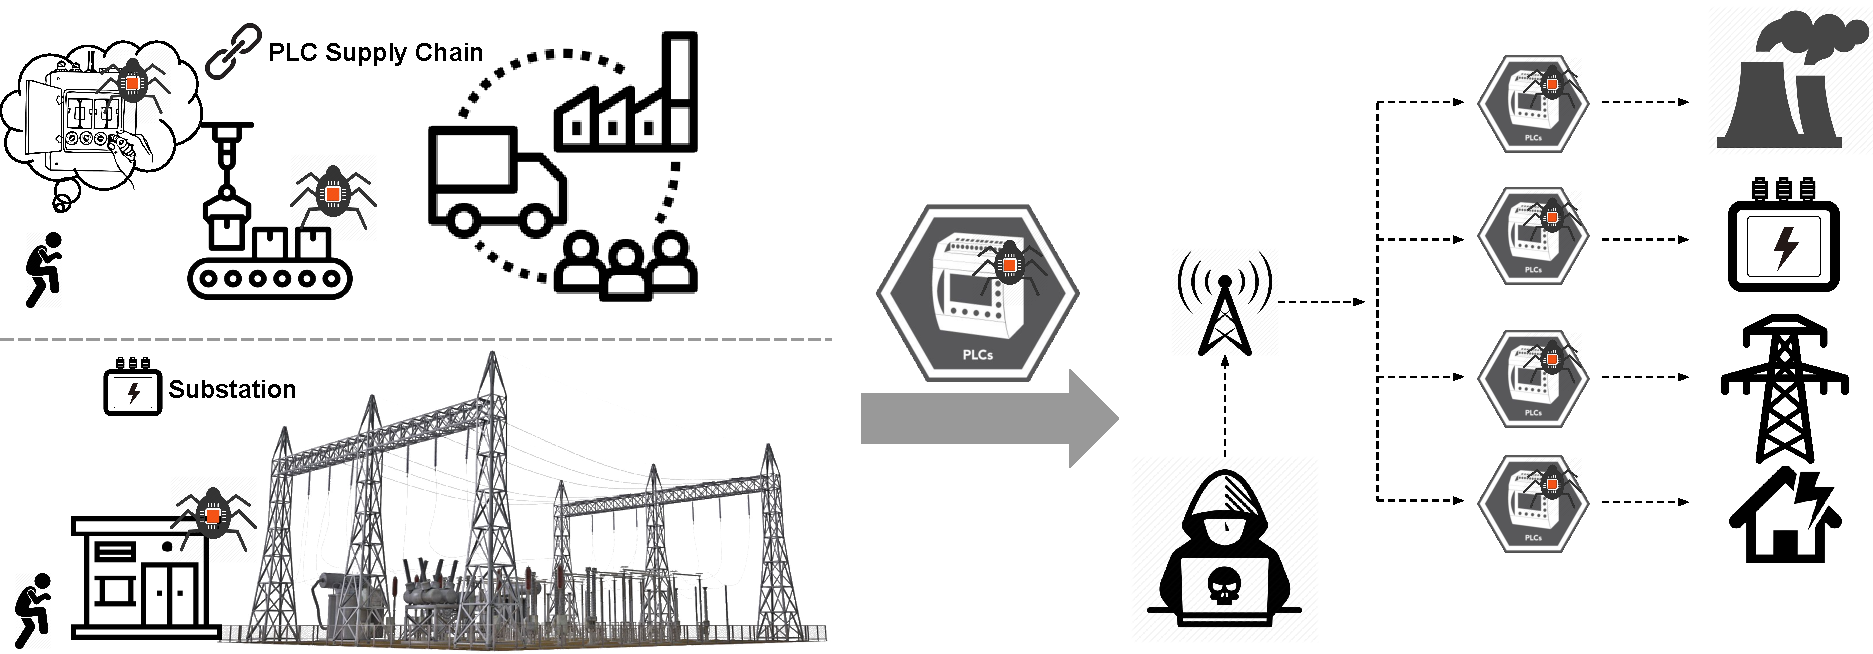
\includegraphics[width=\textwidth]{figures/bigpic}
	\centering
	\caption{Hardware backdoors are installed through industrial control system supply chain penetration of physical contact with industrial systems. Form a botnet that can remotely control multiple points simultaneously.}
	\label{fig:bigpic}
\end{figure*}

